%
% teil7.tex -- Rueckblick und Ausblick
%
\section{Rückblick und Ausblick
\label{komplex:section:rueckblick}}
\kopfrechts{Rückblick und Ausblick}
Diese Arbeit hat am Beispiel des Satzes von Napoleon gezeigt,
wie sich elementare geometrische Aussagen mit komplexen Zahlen behandeln
lassen.
Der Weg führte von der Definition der komplexen Zahlen über die
Polardarstellung und die Drehformel hin zu einem vollständig algebraischen
Beweis eines klassischen geometrischen Satzes.
Was zunächst wie eine künstliche Übersetzung aussieht,
erweist sich bei näherer Betrachtung als die natürliche Sprache für
rotationssymmetrische Probleme.

%
% fig/pdn-quadrat.tex -- Petr-Douglas-Neumann fuer ein Viereck:
% Aus einem beliebigen Viereck A0=ABCD entsteht in zwei Stufen ein Quadrat.
% Stufe 1: Auf jeder Seite gleichschenklig-rechtwinklige Dreiecke nach aussen
% errichten, Spitzen E,F,G,H bilden A1.
% Stufe 2: Die Mittelpunkte der Seiten von A1 bilden das Quadrat A2.
%
% Beispiel:
%   A=(0,0), B=(6,1), C=(7,5), D=(1,6)
%   E=(3.5,-2.5), F=(8.5,2.5), G=(4.5,8.5), H=(-2.5,3.5)
%   M1=(6,0), M2=(6.5,5.5), M3=(1,6), M4=(0.5,0.5)
%
\begin{figure}
\centering
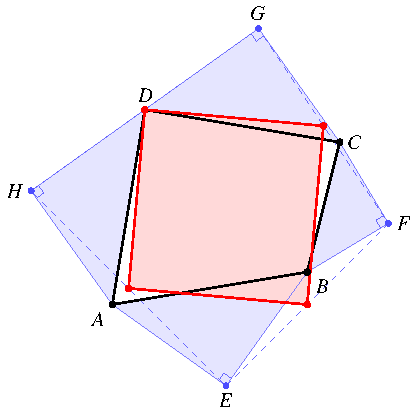
\includegraphics{papers/konstruktion/images/pdn-quadrat.pdf}
\caption{Petr-Douglas-Neumann-Theorem für ein Viereck am Beispiel
$A = 0$, $B = 6 + i$, $C = 7 + 5i$, $D = 1 + 6i$.
Über jeder Seite des Vierecks $ABCD$ (schwarz) wird ein
gleichschenklig-rechtwinkliges Dreieck (rechter Winkel an der Spitze,
markiert) nach aussen errichtet (blau);
die Spitzen $E$, $F$, $G$, $H$ bilden das Viereck $A_1$ (gestrichelt).
Die Mittelpunkte der Seiten von $A_1$ bilden das Quadrat $A_2$ (rot) ---
das Resultat des Verfahrens für $n = 4$.
\label{komplex:figure:pdn-quadrat}}
\end{figure}


Drei Beobachtungen sollen abschliessend hervorgehoben werden.
Erstens wurde der Beweis mit einer einzigen Charakterisierung
gleichseitiger Dreiecke geführt --- Gleichung
\eqref{komplex:eq:charakterisierung} --- und einer einzigen Identität
für den Drehfaktor \eqref{komplex:eq:d-identitaet}.
Diese minimalen Hilfsmittel reichten aus,
um den Satz auf wenige Zeilen Rechnung zu reduzieren.
Zweitens hat sich die Linearität der Konstruktion in den Eckpunkten
als strukturelle Eigenschaft erwiesen, nicht als Zufall.
Sie macht den Satz robust gegenüber Ähnlichkeitstransformationen
und legt nahe, dass ähnliche Resultate für andere symmetrische
Konstruktionen zu erwarten sind.
Drittens trat die geometrische Anschauung an keiner Stelle des Beweises
in den Hintergrund:
Jede algebraische Operation hatte eine konkrete geometrische Deutung,
und umgekehrt.

Die hier vorgestellten Methoden lassen sich auf eine Vielzahl weiterer
Probleme anwenden.
Ein naheliegender Schritt ist die innere Variante des Satzes,
bei der die gleichseitigen Dreiecke nach innen errichtet werden;
auch dort entsteht ein gleichseitiges Dreieck,
dessen Beziehung zum äusseren Napoleon-Dreieck weiterführende Resultate
liefert --- etwa, dass die Differenz der Flächen beider Napoleon-Dreiecke
gleich der Fläche des Ausgangsdreiecks ist.
Verallgemeinerungen führen über regelmässige $n$-Ecke statt gleichseitiger
Dreiecke zum Satz von Petr-Douglas-Neumann.
\index{Satz!von Petr-Douglas-Neumann}%
Abbildung~\ref{komplex:figure:pdn-quadrat} zeigt den Spezialfall $n = 4$ dieses Satzes,
in dem aus einem beliebigen Viereck in zwei Schritten ein Quadrat entsteht.

Weitergehend lassen sich Möbius-Transformationen als spezielle Abbildungen
\index{Mobius-Transformation@Möbius-Transformation}%
der komplexen Ebene studieren, mit denen sich Aussagen über Kreise und
Geraden gleichermassen behandeln lassen; eine ausführliche Darstellung
findet sich im Kapitel~\ref{chapter:moebius} sowie in \cite{komplex:needham} 
und~\cite{komplex:schwerdtfeger}.
Wer den Weg von komplexen Zahlen zu höherdimensionalen Strukturen
weiterverfolgen möchte, gelangt schliesslich zur geometrischen Algebra,
\index{geometrische Algebra}%
die Drehungen, Spiegelungen und Streckungen in beliebiger Dimension in
einem einheitlichen Kalkül zusammenfasst.

Der eigentliche Gewinn dieser Arbeit liegt jedoch nicht im einzelnen
Resultat, sondern in der Methode.
Komplexe Zahlen sind ein Werkzeug, das geometrische Probleme in
algebraische verwandelt --- und damit für Rechnung, Verifikation und
Verallgemeinerung zugänglich macht.
Genau diese Eigenschaft macht sie zu einem unverzichtbaren Bestandteil
des mathematischen Werkzeugkastens.
